\paragraph{�Quienes son?}
Operar estacionamientos es nuestra profesi�n desde 1951. Lo hacemos en centros comerciales, corporativos, clubes de golf, cines, hospitales, hoteles, centros deportivos y universidades en la ciudad de M�xico y quince ciudades m�s.
La piedra angular de nuestro �xito es nuestra reputaci�n de integridad profesional. Ranver es el l�der en esta actividad debido a la atenci�n a todos los aspectos de este negocio, la comprensi�n de las necesidades de los usuarios y propietarios, as� como la aplicaci�n de la m�s avanzada tecnolog�a en el mundo. 

\begin{figure}[h]
	\centering
	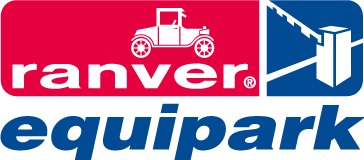
\includegraphics[scale=.3]{./estudioDeMercado/analisisDeLaOferta/source/logo_Ranver}
	\caption{Logo Ranver}
	\label{fig:logo_Ranver}
\end{figure}


A continuaci�n se muestra una cotizaci�n que se hizo en agosto del 2009 con la empresa RANVER S.A DE C.V.

\begin{table}[h]
	\centering
	\rowcolors{2}{grisClaro}{white}
	\begin{tabular}{|l| m{4in}|}
		\hline \textbf{Concepto} & \textbf{Ranver} \\ 
		\hline Recursos Humanos  & M�nimo 2 personas (Cajero, acomodador) \\ 
		\hline Porcentaje de ganancias &  50\% para Ranver y 50\% para el dua�o del estacionamiento, una vez recuperada la inversi�n (entre 1 y  2 a�os)\\ 
		\hline Ventajas & La empresa RANVER cubre todos los gastos en cuesti�n de instalaci�n. \\ 
		\hline Desventajas  & Todo el control del estacionamiento queda bajo la empresa privada y no hay una ganancia para la empresa contratista sino hasta que RANVER haya recuperado su inversi�n. \\ 
		\hline Pago mensual por servicio & La mitad de las ganancias percibidas \\ 
		\hline 
	\end{tabular} 
	\label{tab:cotizacionRanver}
	\caption{Cotizaci�n RANVER}
\end{table}
